
%\subsection{CAD}
\begin{frame}
	\frametitle{CAD to STL}
	\begin{minipage}{0.85\textwidth}
	Tools:
		\begin{itemize}
		\item Create original CAD geometry in CAD program
		\end{itemize}
		\begin{figure}
		
\includegraphics[width=0.4\textwidth]{Pictures/CAD/TUM.png}
		\end{figure}
		Interface:
		\begin{itemize}
		\item Current approach: Export to STL directly.
		\end{itemize}
	\begin{figure}
	%\includegraphics
	\end{figure}
	\end{minipage}
	\begin{minipage}{0.14\textwidth}
		\begin{figure}
					\scalebox{0.08}{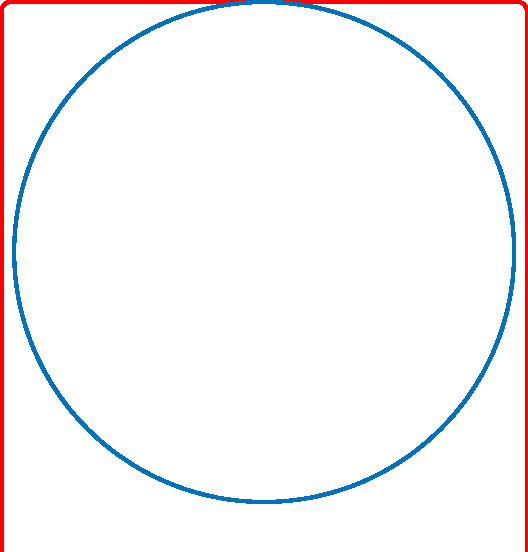
\includegraphics{Pictures/1CADmark.pdf}}\\
					\scalebox{0.08}{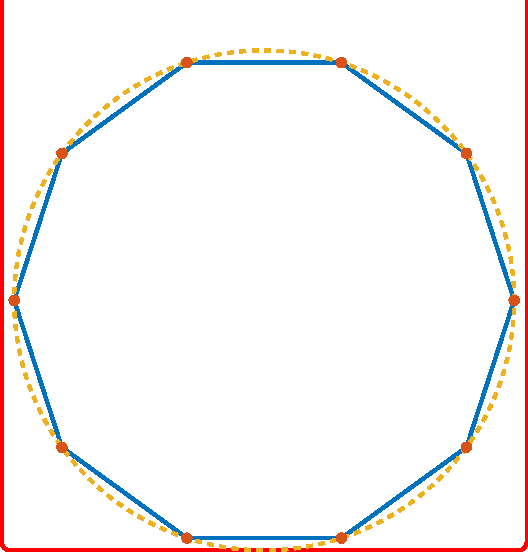
\includegraphics{Pictures/2STLmark1.pdf}}\\
					\scalebox{0.08}{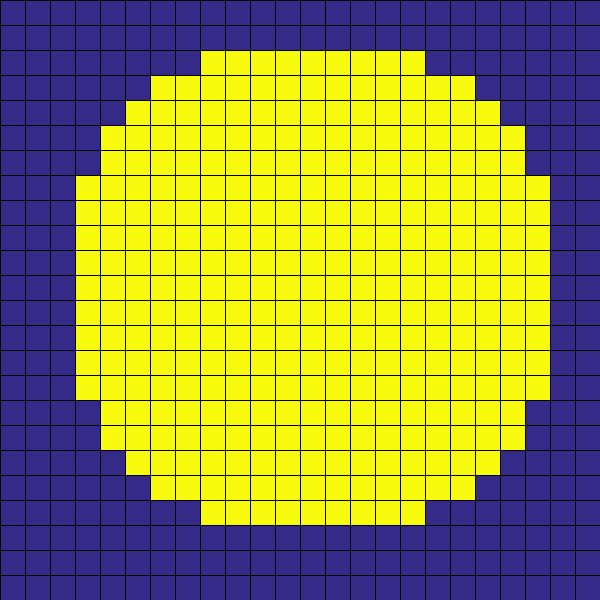
\includegraphics{Pictures/3VOX.pdf}}\\
					\scalebox{0.08}{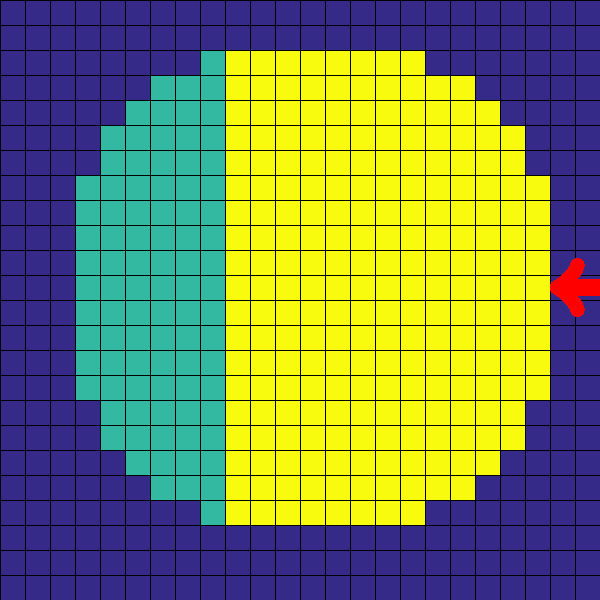
\includegraphics{Pictures/4TPD.pdf}}\\
					\scalebox{0.08}{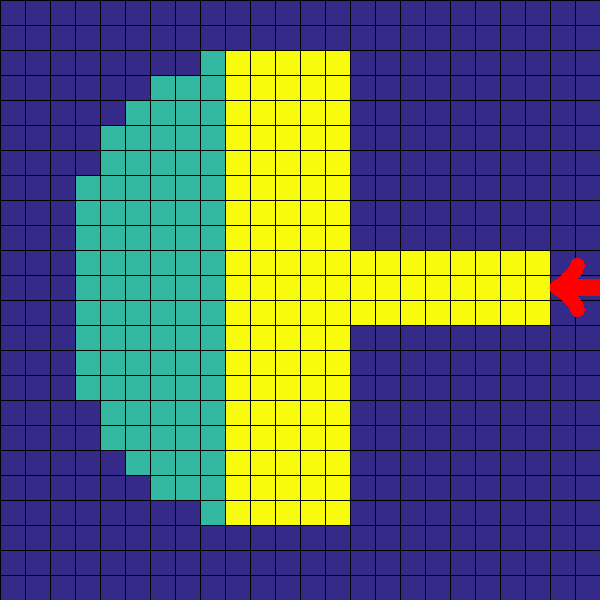
\includegraphics{Pictures/5TOPOPT.pdf}}\\
				%	\scalebox{0.08}{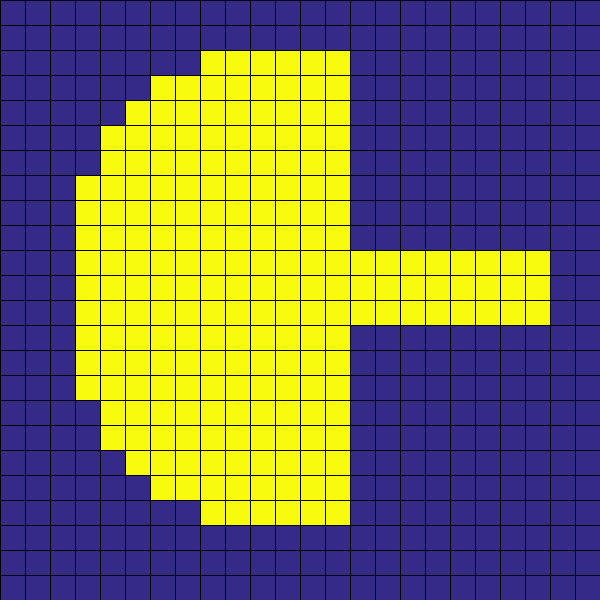
\includegraphics{Pictures/6TOPYOUT.pdf}}\\
					\scalebox{0.08}{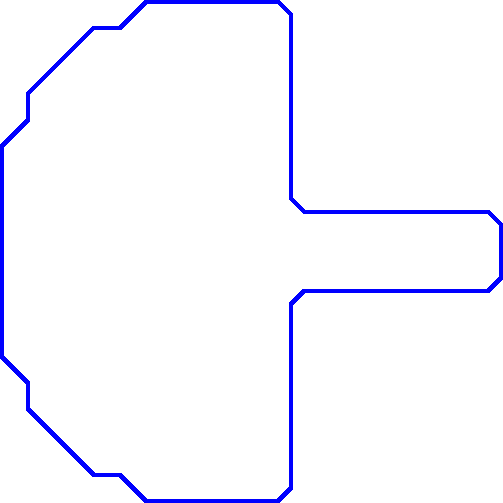
\includegraphics{Pictures/7MC.pdf}}
					\scalebox{0.08}{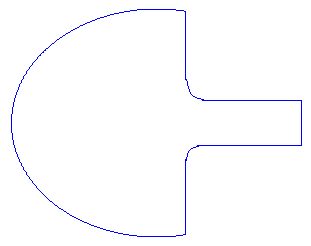
\includegraphics[scale=1.3]{Pictures/End.png}}
		\end{figure}
	\end{minipage}
\end{frame}
%\subsection{STL file}
